\documentclass[aspectratio=169]{beamer}
\usepackage{preamble_beamer}

\newcommand*{\QEDB}{\null\nobreak\hfill\ensuremath{\square}}

\newtheorem*{question*}{Вопрос}
\newtheorem*{claim*}{Утверждение}

\title[Модели стохастической волатильности]{Лекция 6. Локальная волатильность} % The short title appears at the bottom of every slide, the full title is only on the title page

\begin{document}

\begin{frame}
\titlepage 
\end{frame}

\begin{frame}{Модель Блэка-Шоулза}
    Основные предположения:
    \begin{itemize}
        \item Лог-доходности независимы и имеют нормальное распределение
        \item Параметры модели (ставка и волатильность) постоянные или зависят только от времени.
        \item Можно брать кредиты/класть на счёт деньги под одну и ту же ставку $r$
        \item Нет кредитного риска
        \item Непрерывная торговля, без комиссий и market impact
    \end{itemize}
\end{frame}

\begin{frame}{Исторические доходности}
    \begin{itemize}
        \item Определим лог-доходности для реального процесса и геометрического броуновского движения:
        $$
            L_t = \ln \dfrac{S_t}{S_{t-\delta}}
        $$
        \item Визуально очень отличаются:
    \end{itemize}
\begin{figure}
    \centering
    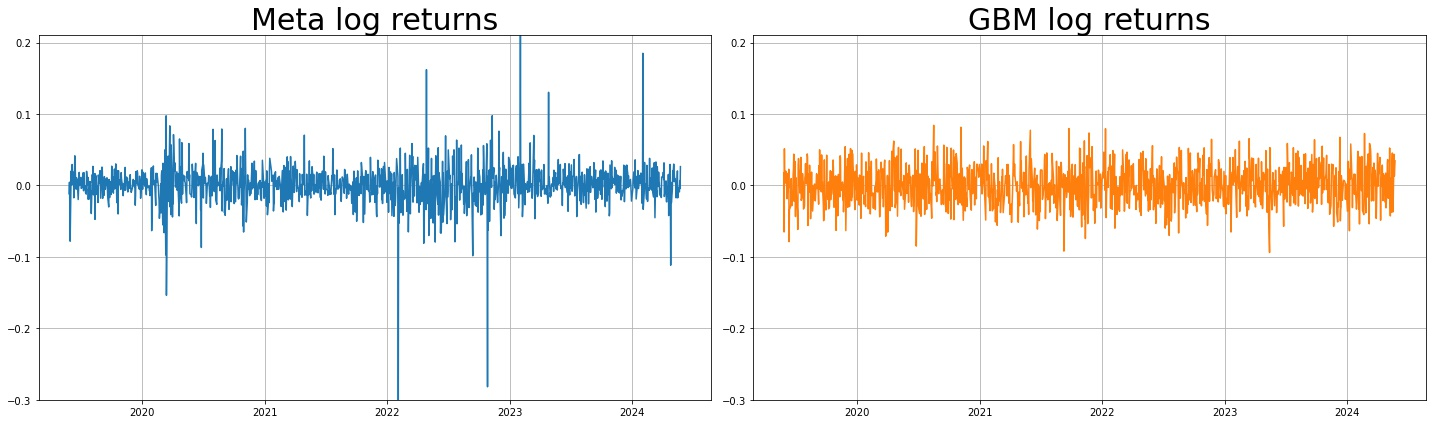
\includegraphics[width=1\linewidth]{6_figs/Meta Log returns plot.jpg}
    \label{fig:enter-label}
\end{figure}
\end{frame}
\begin{frame}{Исторические доходности}
    \begin{itemize}
        \item Исторические доходности имеют толстые хвосты
        \item Коэффициент эксцесса(kurtosis):
            $$
                \kappa = \dfrac{\mathbb{E}\left(L_t-\mathbb{E} L_t\right)^4}{\sigma^4} - 3
            $$
        \item Для нормального $\kappa = 0$, для историчесских данных $\hat{\kappa} \approx 23$. 
    \end{itemize}
    \centering
    \makebox[\textwidth]{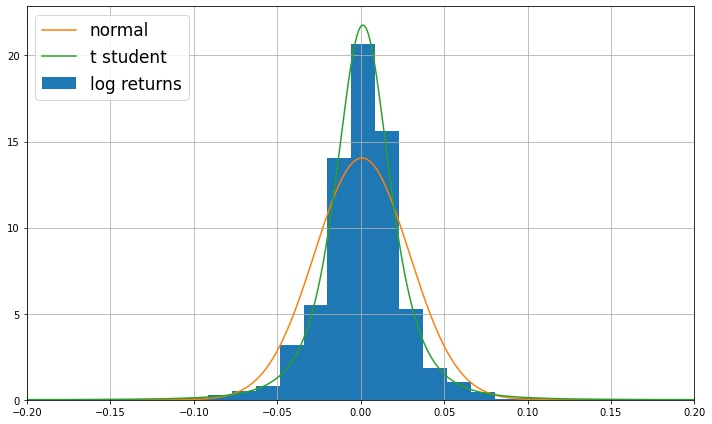
\includegraphics[width=0.5\textwidth]{6_figs/Meta Log returns hist.jpg}}
\end{frame}

\begin{frame}{Исторические доходности}
    \begin{itemize}
        \item Для геометрического броуновского движения:
        $$
            L_t \perp L_{t + s}, \; \forall s \geq \Delta t
        $$
        \item Для рыночных данных:
        $$
            \mathrm{cov}(L_t, L_{t+s}) \approx 0, \;
            \mathrm{cov}(|L_t|, |L_{t+s}|) \neq 0
        $$ 
    \end{itemize}

    \centering
    \makebox[\textwidth]{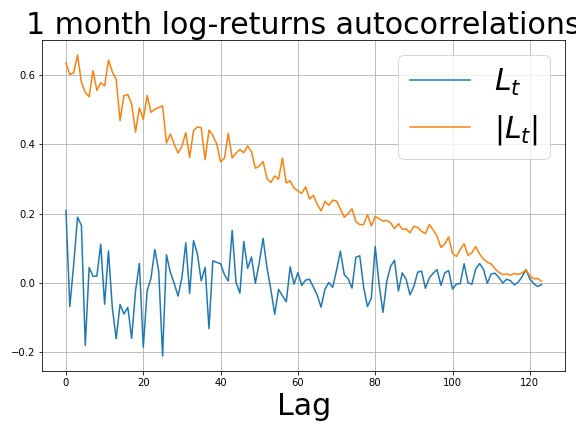
\includegraphics[width=0.4\textwidth]{6_figs/autocorrelation.jpg}}
\end{frame}

\begin{frame}{Другие стилизованные факты}
    \begin{itemize}
        \item Корреляция между волатильностью и ценой
        \item Кластеризация волатильности
        \item Прыжки в доходностях
    \end{itemize}
\end{frame}

\begin{frame}{Вменяемая волатильность}
    \begin{itemize}
        \item Формула Блэка-Шоулза:
        $$
            C_{BS}(S; T, K, r, \sigma) = S \Phi(d_1) - e^{-rT} K \Phi(d_2)
        $$
        \item Знаем рыночные цены $C^{M}(T, K)$, можем решить уравнение относительно $\sigma_{iv}$:
        $$
            C_{BS}(S, T, K, r, \sigma_{iv}) = C^{M}(T, K)   
        $$
        \item В модели Блэка-Шоулза $\sigma_{iv} = \sigma$ -- постоянная. На практике $\sigma_{iv} = \sigma_{iv}(T, K)$.
    \end{itemize}
\end{frame}

\begin{frame}{Вменяемая волатильность}
    \begin{figure}
    \centering
    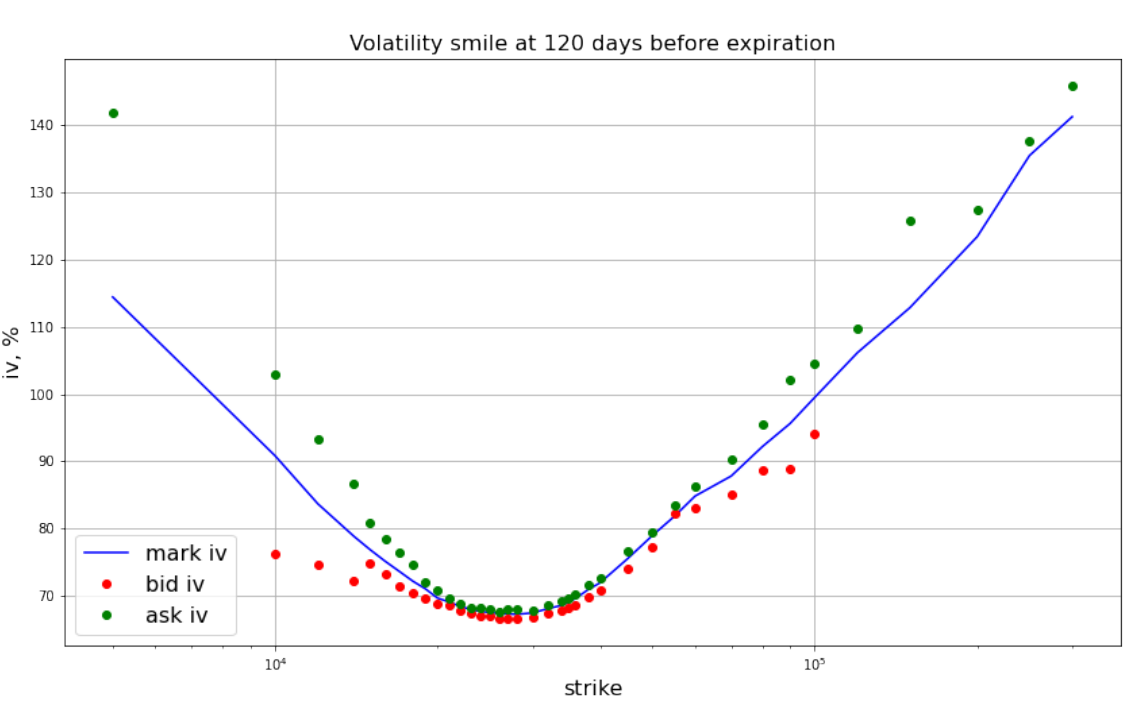
\includegraphics[width=0.8\linewidth]{6_figs/vol smile btc.png}
    \label{fig:enter-label}
\end{figure}
\end{frame}

\begin{frame}{Вменяемая волатильность}
    \begin{itemize}
        \item Как считать $\sigma_{iv}$? Метод Ньютона:
        \only<1>{
            \begin{align*}
                &0 = f(\sigma^*) \approx f(\sigma) + (\sigma^* - \sigma) f'(\sigma) \\
                &\sigma^* = \sigma - \dfrac{f(\sigma)}{f'(\sigma)}
            \end{align*}
        }
        \onslide<2->{
        $$
            {\sigma}_{k+1} = {\sigma}_k - \dfrac{f(\sigma_{k})}{f'(\sigma_k)}
        $$}
        \onslide<2->{\item Здесь 
                $f(\sigma) = C_{BS}(\sigma) - C_{market},  f'(\sigma) = \dfrac{\partial C_{BS}(\sigma)}{\partial \sigma}$}
    \end{itemize}    
\onslide<2->{
    \begin{figure}
        \centering
        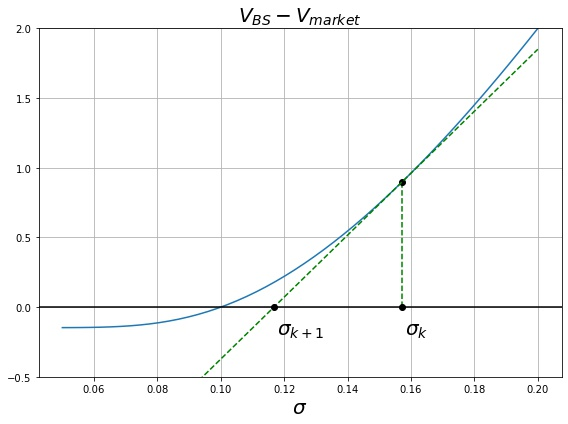
\includegraphics[width=0.43\linewidth]{6_figs/newton.jpg}
        \label{fig:enter-label}
    \end{figure}
}
\end{frame}

\begin{frame}{Модели локальной волатильности}
    \begin{itemize}
        \onslide<1->{\item Пусть динамика процесса задаётся СДУ:
        $$
            \begin{cases} 
            \dfrac{dS_t}{S_t} = r dt + \sigma(t, S_t) dW_t
            \\
            S_0 = s
            \end{cases}
        $$}
        
        \onslide<2->{\item $\sigma(t, S_t)$ -- функция локальной волатильности.}
        \onslide<3->{\item $\sigma(t, S_t) = \sigma(t)$ -- GBM, модель Блэка-Шоулза.}
        \onslide<4->{\item Пример: $\sigma(t, S_t) = \dfrac{\beta}{S_t} \to $
        \begin{align*}
            &dS_t = S_t r dt + \sigma dW_t \\ 
            &S_t = s e^{r t} + \beta \int_0^t e^{r (t-u)} dW_u \sim N(s e^{\mu t}, \ldots)
        \end{align*}}
    \end{itemize}
\end{frame}

\begin{frame}{Формула Бридена-Литценбергера}
    \begin{block}{Теорема}
        Пусть $C(T, K)$ -- цены колл-опционов с датой погашения $T$ и страйком $K$. Тогда риск-нейтральная плотность с.в. $S_T$ задатся формулой:
        $$
            p(T, K) = e^{rT} \dfrac{\partial^2 C(T, K)}{\partial K^2 } 
        $$
    \end{block}
    \textit{Доказательство}
    $$
        C(T, K) = \E^Q e^{-rT} (S_T - K)^+ = 
        e^{-rT} \int_{K}^{\infty}(x-K) p(T, K) dx
    $$
    
    $$
        \dfrac{\partial C(T, K)}{\partial K }
        = e^{-rT} \dfrac{\partial}{\partial K} \left( \int_{K}^{\infty}(x-K) p(T, K) dx \right)
        = -e^{-rT} \int_{K}^{\infty}p(T, K) dx
    $$

    $$
    \dfrac{\partial^2 C(T, K)}{\partial K^2 }
    = e^{-rT} p(T, K)
    $$
\end{frame}

\begin{frame}{Прямое уравнение Колмогорова}
    \begin{itemize}
        \item Риск-нейтральная динамика процесса: 
        $$
            dS_t/S_t = r dt + \sigma(t, S_t) dW_t
        $$

        \item Инфинитизимальный оператор:
        $$
            [Af](t, S) = r S \dfrac{\partial f}{\partial S}
            + \dfrac{1}{2}\sigma^2(t, S_t)S^2 \dfrac{\partial^2 f}{\partial S^2}
        $$

        \item Сопряжённый оператор:
        $$
            [A^*f](t, S) = -r \dfrac{\partial (S f)}{\partial S}
            + \dfrac{1}{2} \dfrac{\partial^2 (\sigma^2(t, S) S^2 f)}{\partial S^2}
        $$

        \item Прямое уравнение Колмогорова:
        $$
            \dfrac{\partial p}{\partial t} = [A^*f](t, S)
            = -r \dfrac{\partial (S p)}{\partial S}
            + \dfrac{1}{2} \dfrac{\partial^2 (\sigma^2(t, S) S^2 p)}{\partial S^2}
        $$
    \end{itemize}
\end{frame}

\begin{frame}{Формула Дюпира}

    \begin{block}{Формула Дюпира}
        Пусть RN-динамика процесса $S_t$ задаётся моделью локальной волатильности:
        $$
            dS_t / S_t = r dt + \sigma(t, S_t) dW_t
        $$
        Тогда поверхность цен колл-опционов $C(T, K)$ удовлетворяет уравнению: 
        $$
            \dfrac{\partial C}{\partial T} = \dfrac{1}{2} \sigma^2(T, K) K^2 
            \dfrac{\partial^2 C}{\partial K^2} - r K \dfrac{\partial C}{\partial K}
        $$
        В частности, если $C^M(T, K)$ -- рыночная поверхность цен опционов, и
        $$
            \sigma^2_{Dup}(t, S) = \left.\dfrac{\frac{\partial C^M}{\partial T} + r K \frac{\partial C^M}{\partial K}}
            {K^2 \frac{\partial^2 C^M}{\partial K^2}} \right\vert_{T=t, K=S}
        $$то модель точно описывает рыночные цены.
    \end{block}
\end{frame}

\begin{frame}{Формула Дюпира: доказательство}
    \begin{itemize}
        \item Общая формула ценообразования:
        $$
            C(T, K) = \E^Q (S_T - K)^+ = \int_{K}^{\infty} (x-K) p(T, x) dx
        $$
        \item Вычислим производную по $T$:
        \begin{align*}
            &\dfrac{\partial C}{\partial T} =  
            \int_{K}^{\infty} (x-K) \dfrac{\partial p(T, x)}{\partial T} dx = [\text{Уравнение Колмогорова}]\\ 
            & =\dfrac{1}{2} \int_{K}^{\infty} (x-K) \dfrac{\partial^2 (x^2 \sigma(T, x) p(T, x))}{\partial x^2} dx = [\text{по частям}]\\
            & =-\dfrac{1}{2} \int_{K}^{\infty} \dfrac{\partial (x^2 \sigma(T, x) p(T, x))}{\partial x} =\dfrac{1}{2} K^2 \sigma(T, K) p(T, K)
        \end{align*}
        \item По формуле Бридена-Литценбергера:
        $$
            p(T, K) = \dfrac{\partial^2 C(T, K)}{\partial K^2} 
        $$\QEDB
    \end{itemize}
\end{frame}

\begin{frame}{Связь с implied volatility}
    \begin{itemize}
        \only<1>{\item Log moneyness: 
        $$
            k = \ln(\frac{K}{S_0e^{rT}})
        $$
        \item Total variance:
        $$
            \omega(T, k) = T \sigma_{iv}^2(T, S_0e^{rT+k})
        $$
        \item Формула Блэка-Шоулза:
        $$
            C_{BS}(T, K) = S_0 \left( N\left(-\frac{k}{\sqrt{\omega}} + \dfrac{1}{2}\sqrt{\omega}\right)
             - e^{k} N\left(-\frac{k}{\sqrt{\omega}} - \dfrac{1}{2}\sqrt{\omega}\right) \right)
        $$}
        \only<1->{
        \item Формула Дюпира:
        $$
            \sigma_{Dup}^2(T, K) = \dfrac{\frac{\partial \omega}{\partial T}}
            {1 - \frac{k}{\omega} \frac{\partial \omega}{\partial k} + 
            \frac{1}{4}(-\frac{1}{4} + \frac{1}{\omega} + \frac{k^2}{\omega^2}) (\frac{\partial \omega}{\partial k})^2 + 
            \frac{1}{2} \frac{\partial^2 \omega}{\partial k^2}}
        $$}
        \only<2>{
            \centering
            \makebox[\textwidth]{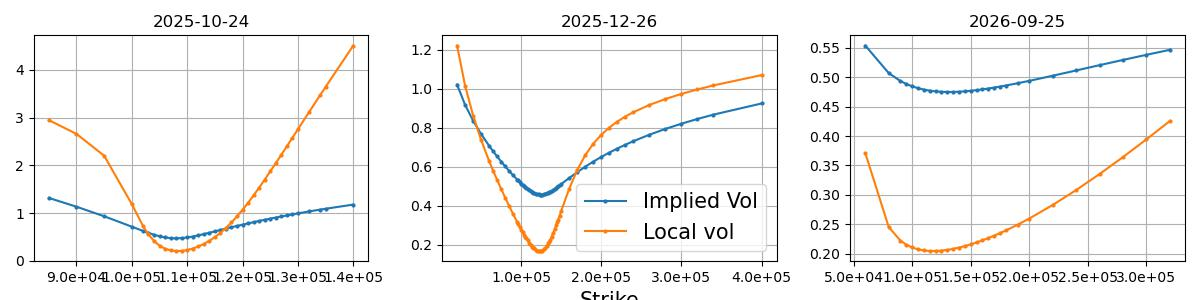
\includegraphics[width=1\textwidth]{6_figs/local_vs_implied.jpg}}
        }
    \end{itemize}
\end{frame}

\end{document}
